
\chapter{Eletrônica}

Para solucionar o problema da implementação de um radar de efeito \emph{doppler}  foi estipulado uma solução dividida em vários sistemas integrados, onde todos esses sistemas estariam dentro de um totem dispostos de acordo com a Figura \ref{esquematico1}. Nesta disposição a solução está dividida em, sistema do radar,  sistema de processamento de sinais, sistema de controle e sistema de comunicação.


\begin{figure}[H]
    \centering
    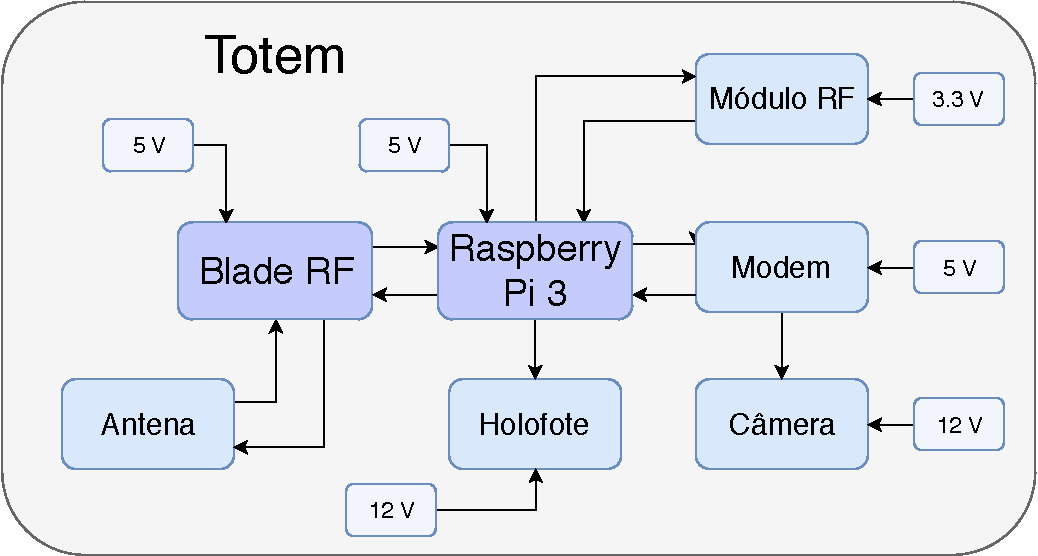
\includegraphics[scale=0.85]{totem.pdf}
    \caption{Esquemático da solução eletrônica proposta para a construção do totem. }
    \label{esquematico1}
\end{figure}

\section{Sistema do radar}

O radar será implementado na configuração monoestática, isto é, será utilizado apenas uma  antena para realizar a transmissão e recepção do sinal. Devido a este fator, foi escolhido a modulação  \emph{ Frequency shift keying - FSK} utilizando um sinal de controle do tipo \emph{Pulse Width Modulation} (PWM), para realizar a transmissão de modo que haja um intervalo entre a emissão e captação dos pulsos. Portanto, uma fração do período de repetição dos pulsos corresponderão a uma janela de tempo para a \emph{Field Programable Array} (FPGA) processar a informação recebida da antena, e a outra parte para enviar o sinal. Esse tipo de configuração foi escolhida pela diminuição dos custos do projeto.
Nas próximas seções referentes ao radar, estarão detalhados os blocos do diagrama da Figura \ref{processos_geral_radar}, onde cada bloco será expandido para explicar seu funcionamento.

\begin{figure}[H]
    \centering
    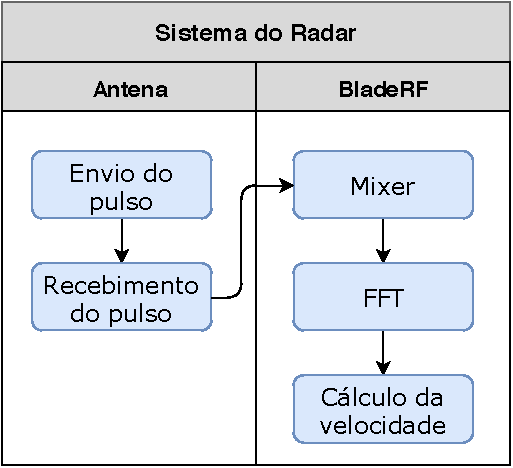
\includegraphics[scale=1]{sistema_radar.pdf}
    \caption{Diagrama geral do radar representando a responsabilidade de cada bloco na detecção do veículo e estimativa da velocidade.}
    \label{processos_geral_radar}
\end{figure}

\subsection{Parâmetros do radar}

O projeto consiste em transmitir e receber um sinal para detectar a aproximação de um veículo, e após detectar, analisar o desvio de frequência para estimar sua velocidade. Para realização deste processo, é preciso definir alguns parâmetros para realização dos cálculos.

O primeiro parâmetro é a distância máxima que o radar vai conseguir captar um veículo. A partir disso foi estipulado uma distância de 100m, visto que com essa distância é possível alertar o motorista que vem em sentido contrário, além de dar tempo para que seja possível capturar uma imagem se o veículo estiver acima da velocidade da via. A partir disso foi possível realizar o cálculo dos demais parâmetros.

Após isso foi calculado a frequência de repetição de pulso \emph{ (Pulse Repetition Frequency - PRF)},  que é o número de ciclos de transmissão e é calculado por:
\begin{equation}\label{R_MAX}
    R_{max} =  \frac{c}{2PRF},
\end{equation}
onde \emph{c} é a velocidade da luz e $R_{max}$ é a distância máxima de alcance do radar. Com isso temos que a PRF é de:
\begin{equation}\label{PRF}
  PRF =  \frac{c}{2R_{max}} = \frac{3.10^8}{2.100} = 1.5MHz.
\end{equation}

Já o intervalo de repetição do pulso \emph{(Pulse Repetition Interval - PRI)} é o inverso da PRF que nesse caso é de $0.6\mu s$. Através desse intervalo de tempo podemos determinar o tempo de transmissão do pulso que é dado através de: 
\begin{equation}\label{duty}
  d_t = \tau . PRF,
\end{equation}
onde $d_t$ é o \emph{duty cicle} ou largura do pulso e $\tau$ é o tempo de transmissão do pulso. Considerando que o \emph{duty cicle} é de 50$\%$, ou seja, o pulso será mandado na metade do tempo e na outra metade será recebido, o tempo de transmissão é:
\begin{equation}\label{tal}
  \tau = \frac{d_t}{PRF} =  \frac{0.5}{1.510^6} = 0.33\mu s.
\end{equation}
%%%%%%%%%parametrôs de potencia e ruido%%%%%%%%%%%%%%
A relação a seguir define a potência a ser recebida em função de diversos parâmetros:
\begin{equation}\label{potencia_recebida}
    P_r\, =\,    \frac{P_{t}\,\, G^{2}\,   \lambda^{2}\, \sigma }{(4\pi)^{3}\,  R^{4}} 
\end{equation}%
Onde $P_r$ é a potência recebida, $P_t$ a potência transmitida, $G$ o ganho da antena, $\lambda$ o comprimento de onda do sinal a ser enviado, $\sigma$ a área de seção transversal média do alvo e $R$ a distância do alvo até a antena.

A potência máxima a ser transmitida pelo \emph{Software Defined Radio - SDR} é de 6 dBm, considerando neste valor a distância de 100 m , o ganho da antena que é de 9 dB, o comprimento de onda para a transmissão do pulso a 915 MHz que corresponde a 0,328 m e uma seção média de 1 $m^2$ a relação \ref{potencia_recebida}.

Através das informações acerca do CI LMS6002 a sensitividade na entrada do receptor é de -116 dBm.
% descrever um caso de funcionamanto do radar para ilustrar a situação  

\subsection{Antena}
A antena utilizada no projeto é uma antena dipolo com frequência central a 915 MHz e com uma largura de banda de 26 MHz. A Figura \ref{antena} mostra a antena que será utilizada. Sua polarização é linear. 

\begin{figure}[H]
    \centering
   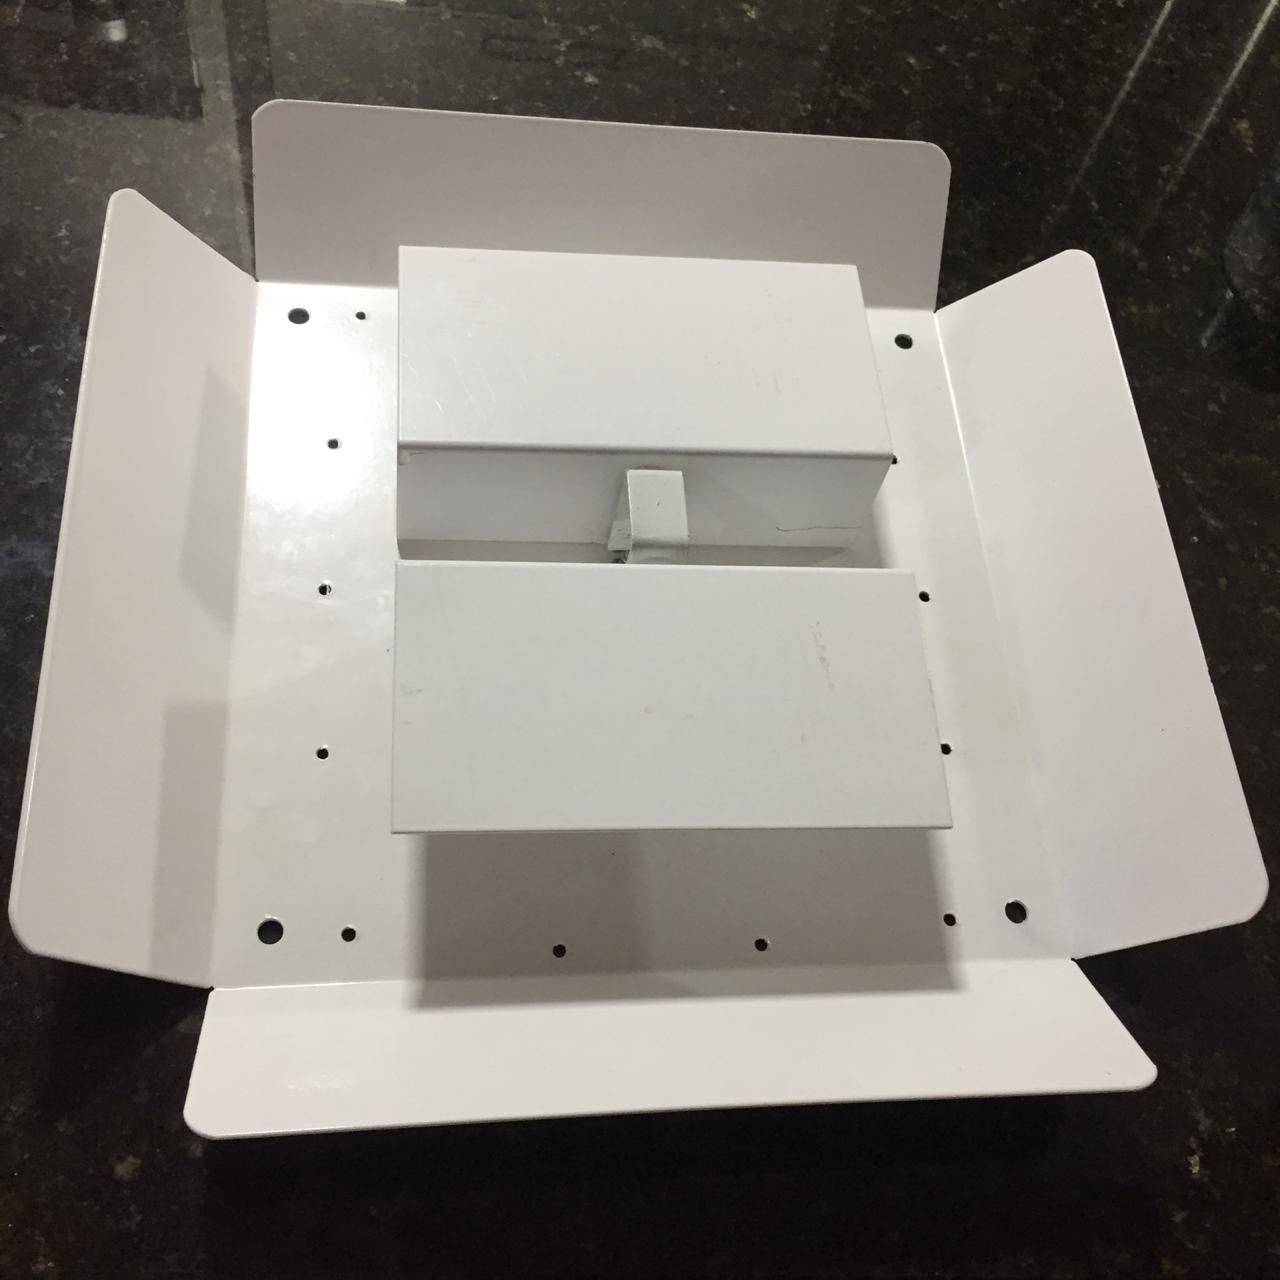
\includegraphics[scale = 0.15]{antena.jpeg}
   \caption{Antena dipolo com frequência central de 915MHz, que será utilizada para a transmissão e recepção de dados no radar.}
   \label{antena}
    \end{figure}

Outros parâmetros importantes da antena são sua diretividade, ou seja, a capacidade de focalizar energia em um ponto, e também o ganho da antena. Neste caso a antena possui um ganho e diretividade de 9dB como mostrado na Figura \ref{ganho}.

\begin{figure}[H]
    \centering
   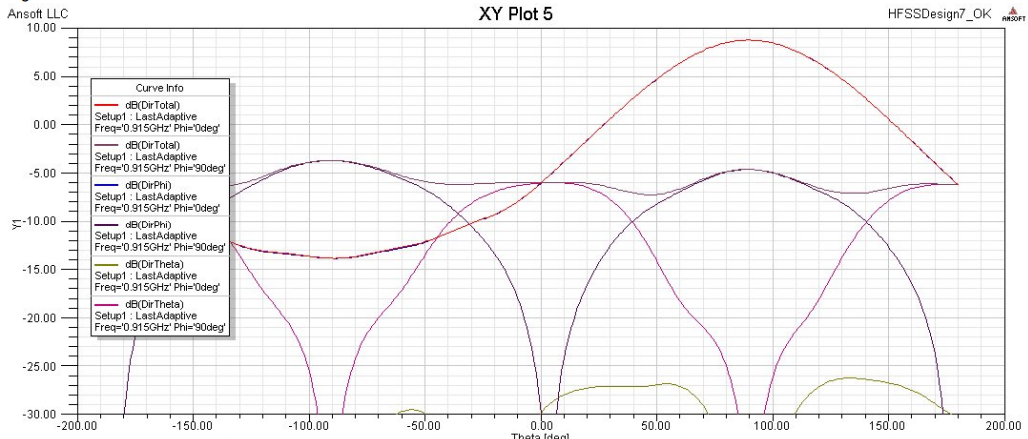
\includegraphics[scale = 0.5]{ganho.png}
   \caption{Diagrama de radiação com o ganho da antena.}
   \label{ganho}
    \end{figure}

Podemos verificar também a abertura 3dB da antena, onde está concentrado metade da energia transmitida ou recebida pela antena.  Para calcular este ângulo é preciso pegar o maior valor no diagrama de radiação e baixar 3dB. Na Figura \ref{dr} mostra que a abertura angular é de $60^o$

\begin{figure}[t]
    \centering
   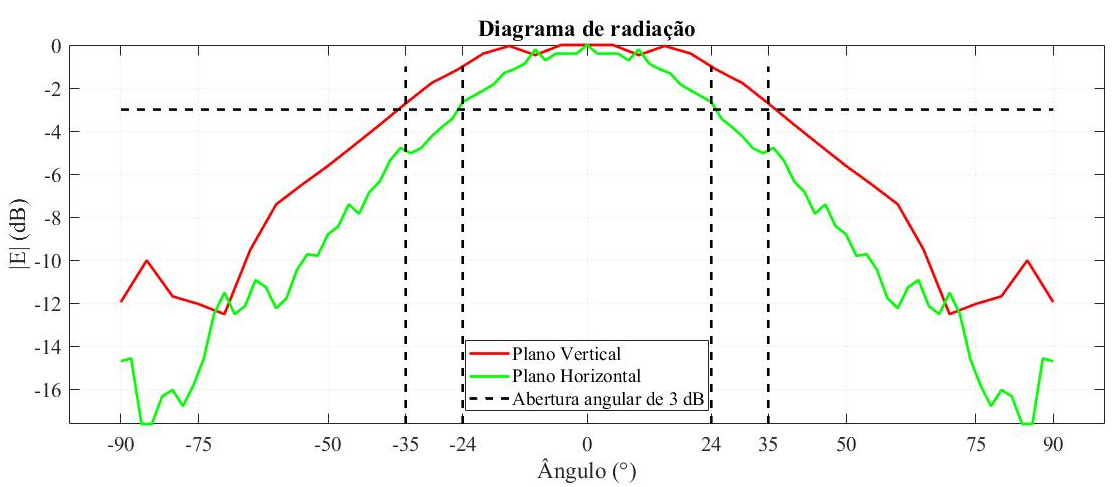
\includegraphics[scale = 0.35]{gir.png}
   \caption{Diagrama de radiação da antena e a
abertura 3dB.}
   \label{dr}
    \end{figure}


\subsection{Processamento de sinais}
 
O processamento de sinal realizado dentro do radar consiste em realizar a transmissão e recepção do sinal dentro da \emph{BladeRF}, visto na Figura \ref{bladerf}, utilizando o FPGA \emph{Cyclone IV}, de modo que se possa calcular com a frequência central na recepção a velocidade do veículo que se aproxima da curva. 

\begin{figure}[H]
    \centering
   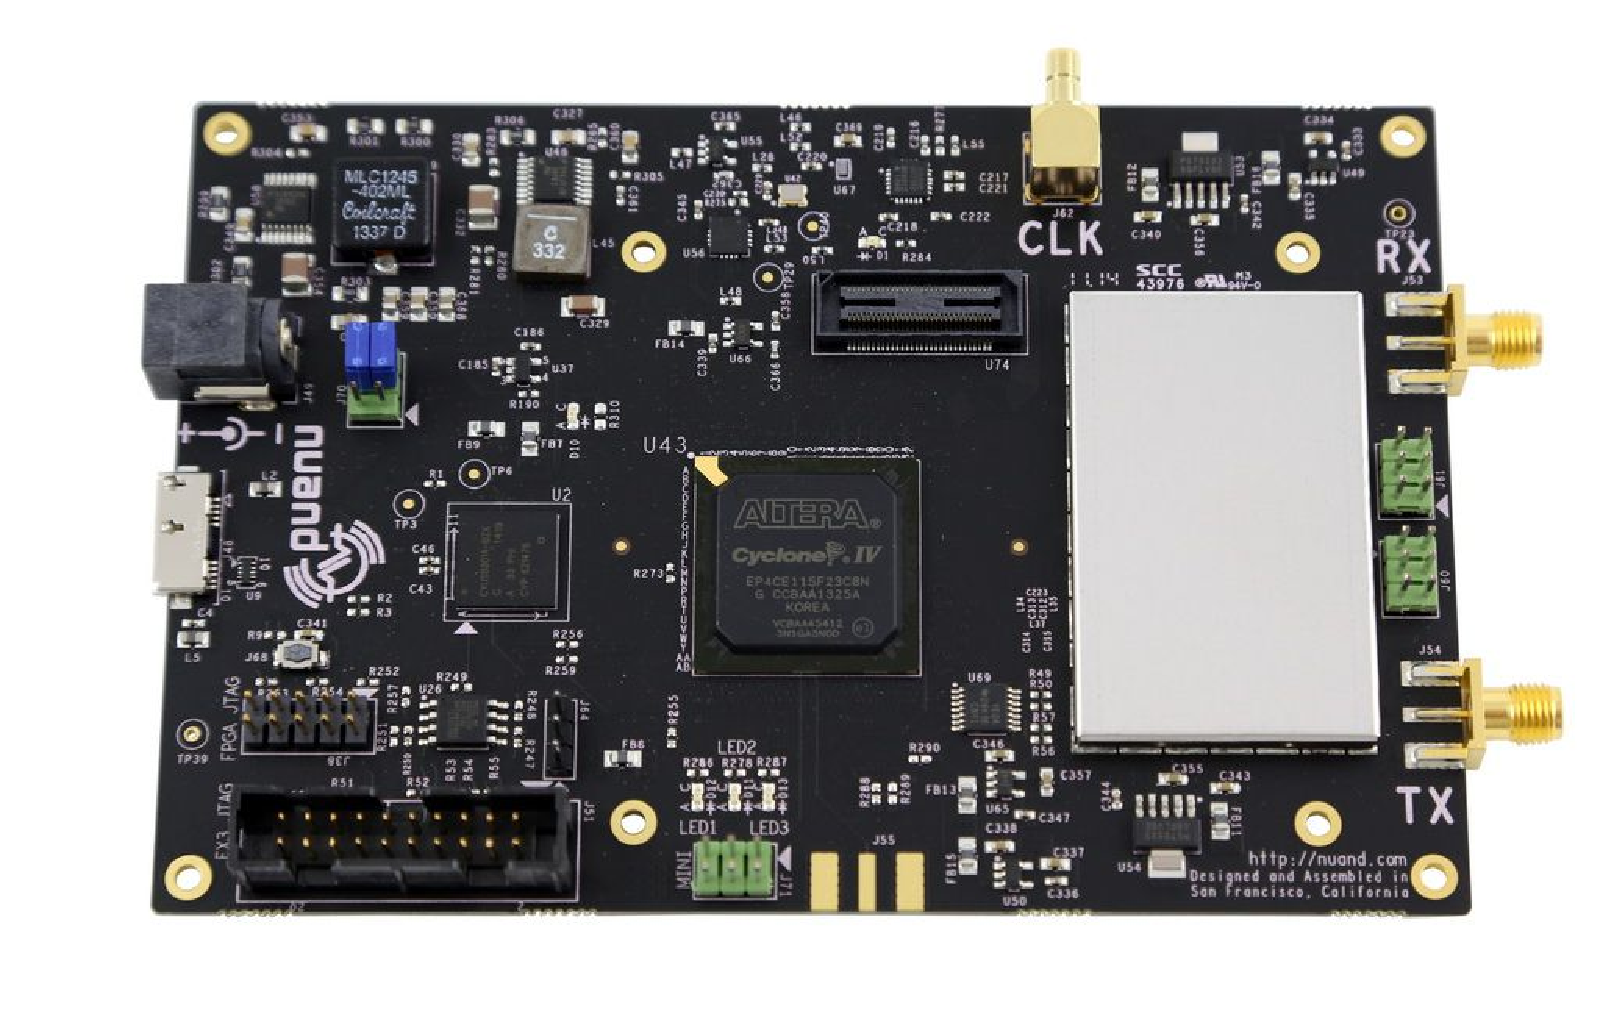
\includegraphics[scale = 0.4]{bladerf.pdf}
   \caption{Placa de rádio definido por \emph{software Nuand BladeRF x115} que realizará a transmissão e recepção do sinal e o cálculo de velocidade do veículo.}
   \label{bladerf}
    \end{figure}

Para realizar a transmissão do sinal é realizado uma modulação que consiste em uma multiplexação de dois sinais, uma senoide com frequência em 915 MHz e um sinal DC ligado ao \emph{ground} de modo que um pulso PWM realizaria o controle da saída do sistema, realizando assim uma modulação FSK.

Na recepção do sinal é feito primeiramente sua \emph{Fast Fourier transform (FFT)}, e em sequência o sinal passa por um filtro que tem como intuito limpar o espectro do sinal, retirando assim as baixas frequências possibilitando caracterizar em que frequência central encontra-se o sinal refletido pelo veículo. Uma vez que se sabe a frequência do sinal recebido, o mesmo passa por um algoritmo que tem como função implementar a equação de efeito \emph{doppler} para o desvio de frequência:
\begin{equation}\label{freq_desv}
  \Delta f = \frac{\Delta v}{c}f_o.
\end{equation}

Isolando a variável $\Delta v$, encontra-se a seguinte relação para o desvio de velocidade:
\begin{equation}\label{vel}
  \Delta v = \frac{\Delta f c}{f_o},
\end{equation}

Onde $\Delta f$ é o desvio de frequência com relação a frequência central, $\Delta v$: é o desvio de velocidade com relação ao desvio de frequência, \emph{c} é a velocidade da luz e $f_o$ é a frequência central do sinal. Uma vez implementado o algoritmo com a equação do efeito \emph{doppler} é possível encontrar a velocidade do veículo.

\subsubsection{Desvio mínimo de frequência para resolução da FFT}

 Considerando a relação da equação \ref{freq_desv}, um desvio equivalente a 1 $km/h$ corresponde a um desvio de frequência da ordem de 2 $Hz$ o que corresponde a resolução mínima para a FFT. Essa resolução de velocidade será suficiente para realizar a análise dos veículos que estarão travegando sobre a via.%Colocar mais coisa 
 \subsubsection{Taxa de repetição de pulso e período de repetição de pulso}
 
 % duty cycle e interferência na latência máxima para determinar a velocidade
 
\subsubsection{Métodos de melhoramento da SNR}%(add ao diagrama)
%integração coerente
A SNR pode ser melhorada através da soma de N pulsos recebidos pela antena, utilizando esta técnica conhecida como integração, %[livro do richard]
e aumentando a SNR por um fator de N.


\subsection{Arquitetura}

Para realizar a solução proposta para recepção e transmissão do sinal foi verificado qual a arquitetura padrão utilizada pelo fabricante, que está representada na figura \ref{arquitetura}. Após isso foi adicionado as soluções abordadas nessa seção de modo que a arquitetura do sistema ficou de acordo com o que está representado no anexo  Figura \ref{arquitetura1}. As alterações propostas tem o intuito de realizar a transmissão e recepção da mensagem.
\begin{figure}[H]
    \centering
   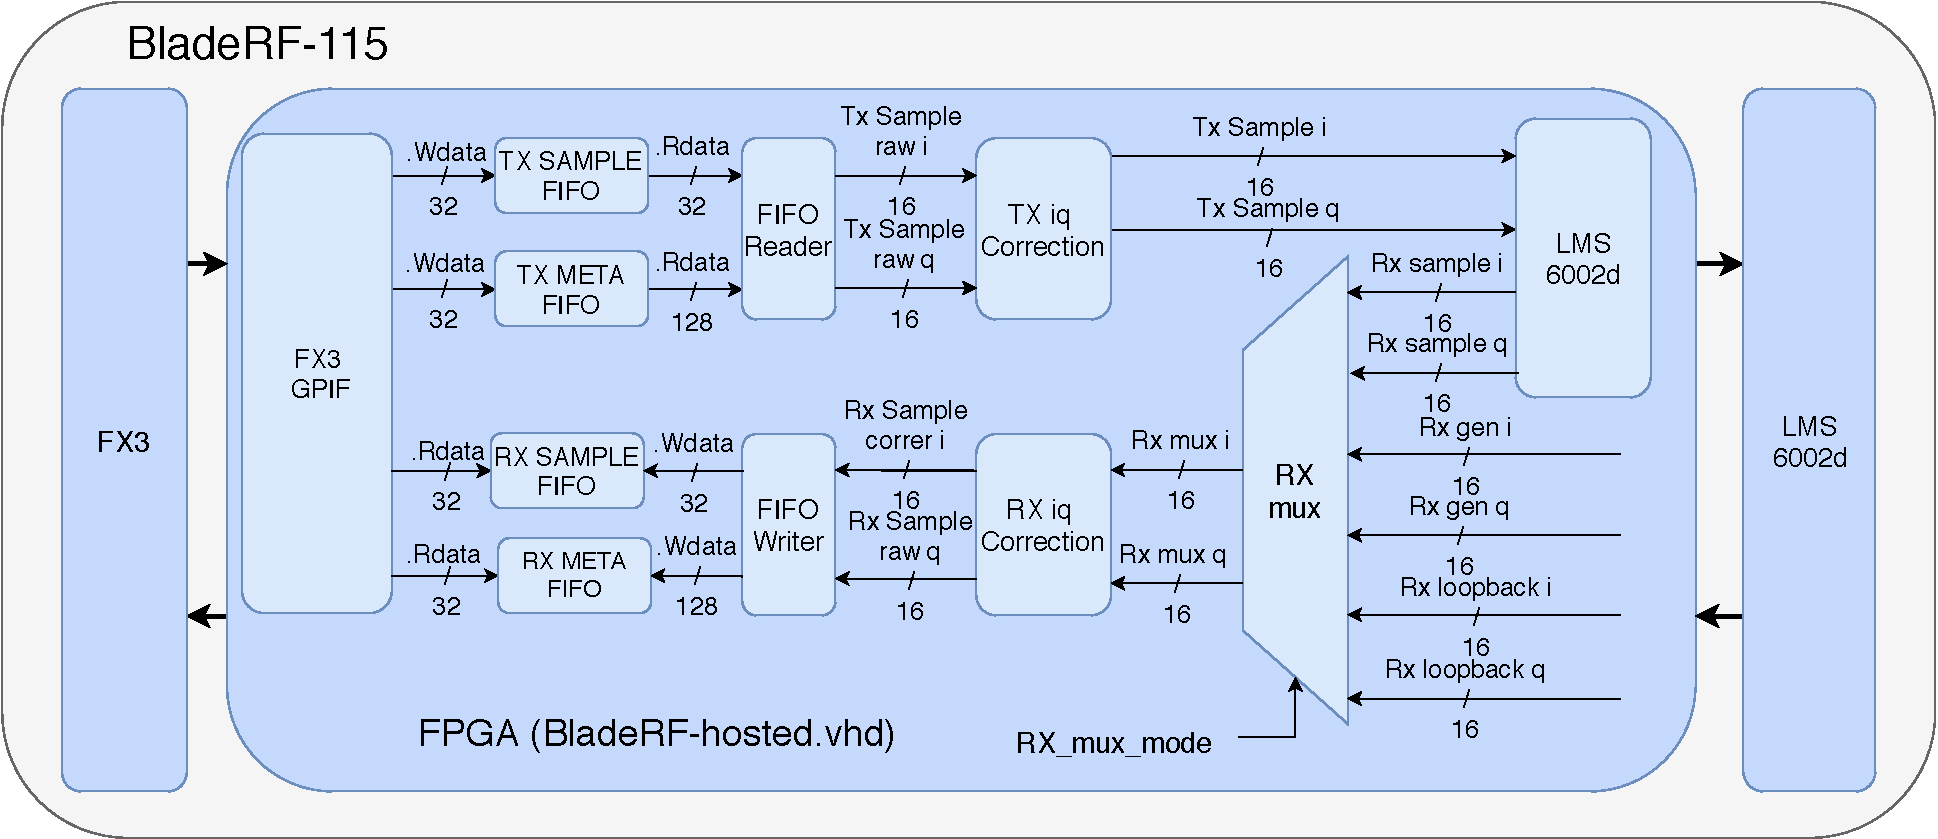
\includegraphics[scale = 0.48]{blade.pdf}
   \caption{Arquitetura utilizada pelo fabricante para emissão e recepção do sinal.}
   \label{arquitetura}
    \end{figure}
    
        
\section{Sistema de controle}
    O sistema de controle tem como função principal realizar o processamento, monitoramento e comunicação dos vários módulos presentes no projeto. A implementação desse sistema de controle embarcado consiste em um microcontrolador, que para o caso do projeto foi modelado tendo em vista a placa de desenvolvimento \emph{Raspberry Pi 3}, como mostra a Figura \ref{raspberry}, sendo esta escolhida pelo seu alto desempenho com relação ao tempo de processamento dos sinais que serão enviados e também por apresentar um bom custo-beneficio com relação ao que é requisitado para o projeto. 
    
    \begin{figure}[H]
    \centering
   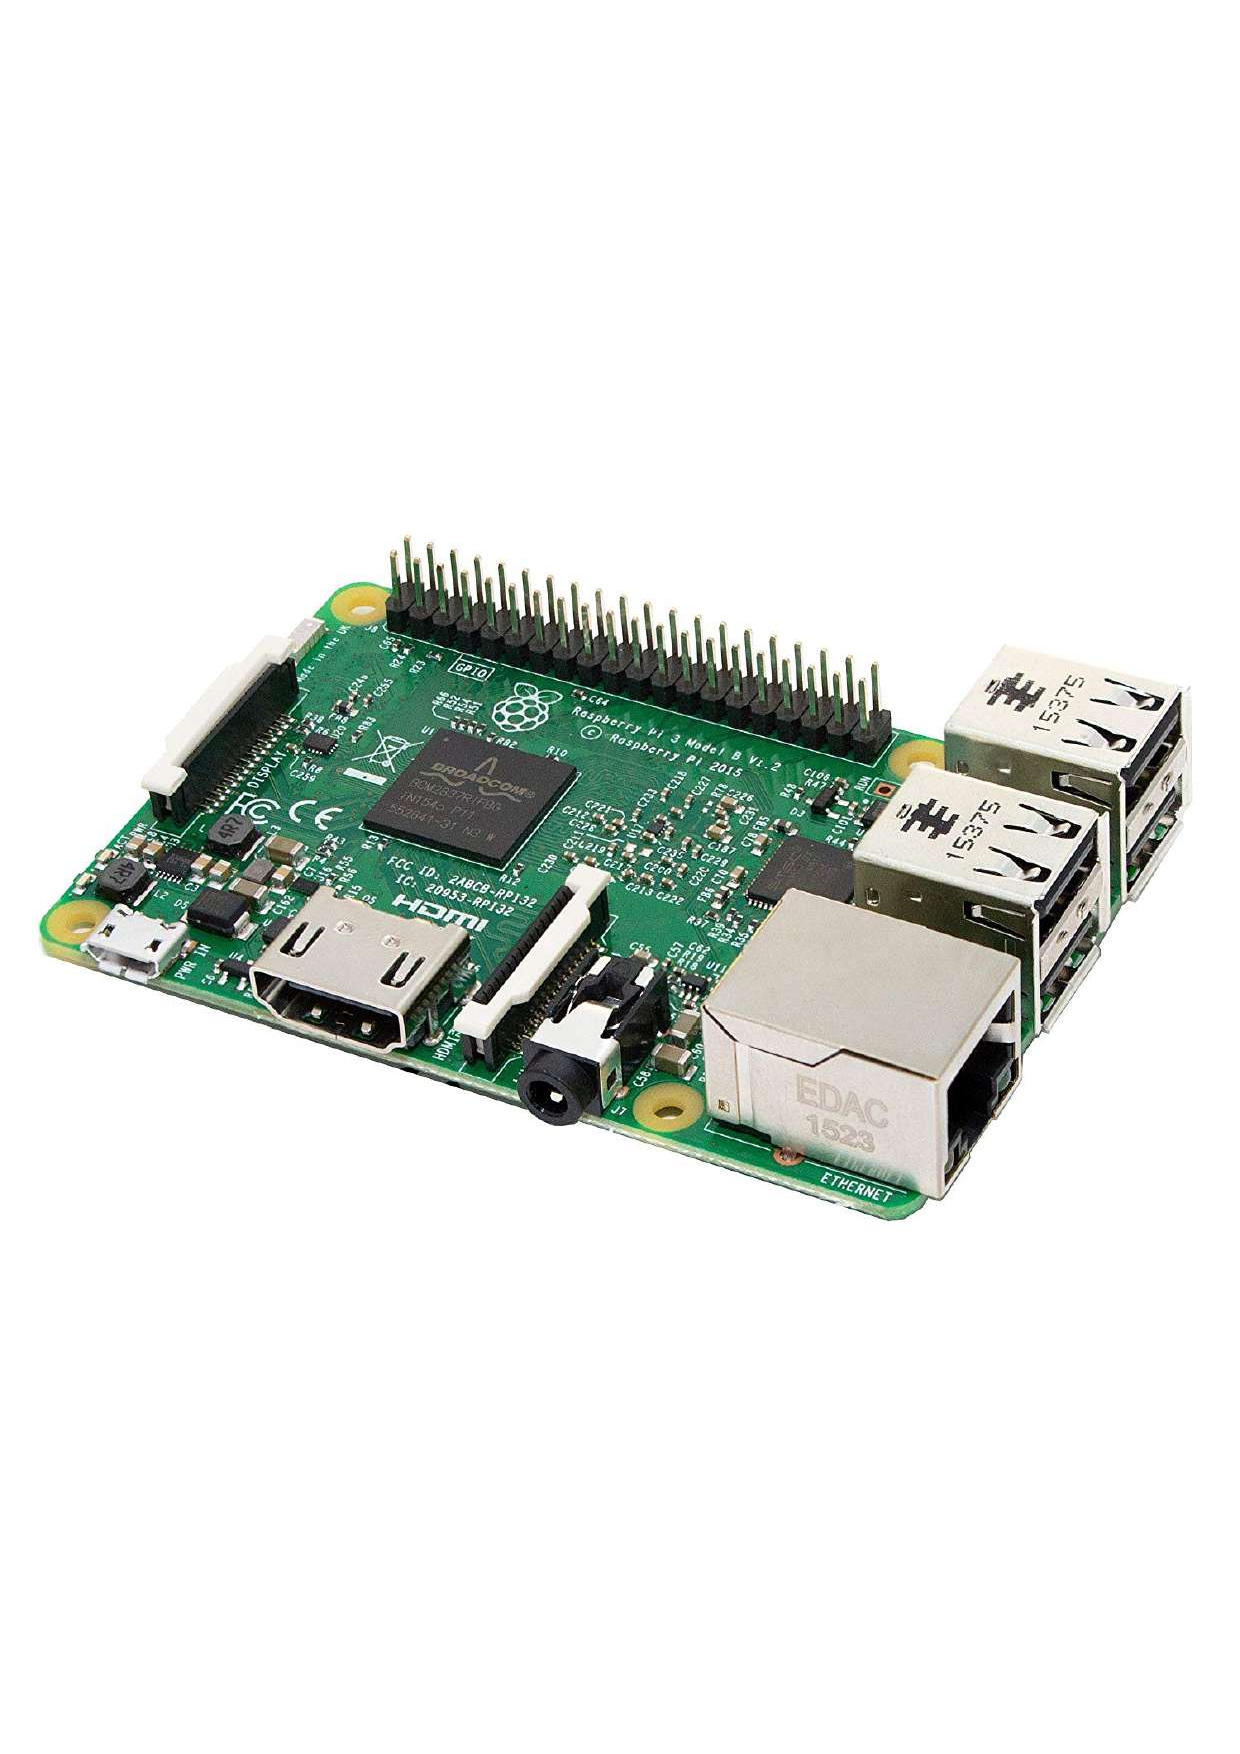
\includegraphics[scale = 0.27]{raspberry.pdf}
   \caption{Placa \emph{Raspberry PI 3} que será responsável por fazer o controle dos módulos e o processamento da imagem.}
   \label{raspberry}
    \end{figure}
    
    
    \subsection{Tempo de latência}
    Dentre os principais requisitos solicitados pela placa é que a mesma possui uma latência máxima de operação para se comunicar entre os módulos de aproximadamente 2.68 s, sendo este dado obtido através do tempo que um veículo com velocidade máxima de 150 km/h ou aproximadamente 41 m/s usaria para percorrer a distância do ponto de captura de sua velocidade até o ponto onde ocorre a captura da imagem casso ocorra uma infração. 
    
    \subsection{Detecção do veículo e iluminação}
    Este sistema é responsável por enviar ao totem que se encontra na via no sentido contrário uma \emph{flag} quem tem como objetivo avisar que foi detectado um veículo vindo em sua direção, e consequentemente o totem no qual foi enviado a \emph{flag} aciona um aviso luminoso ao condutor para ter uma atenção redobrada na curva. A \emph{Raspberry} recebe do rádio \emph{BladeRF} a informação de detecção do veículo e a partir do módulo NRF24L01, visto na Figura \ref{nrf24}, transmite para o outro totem, que com o mesmo módulo faz a recepção da informação. Ao receber esta informação, é acionado um relé para ligar o aviso luminoso, que alertará o condutor sobre um veículo se aproximando na direção contrária.
    
    \begin{figure}[H]
    \centering
    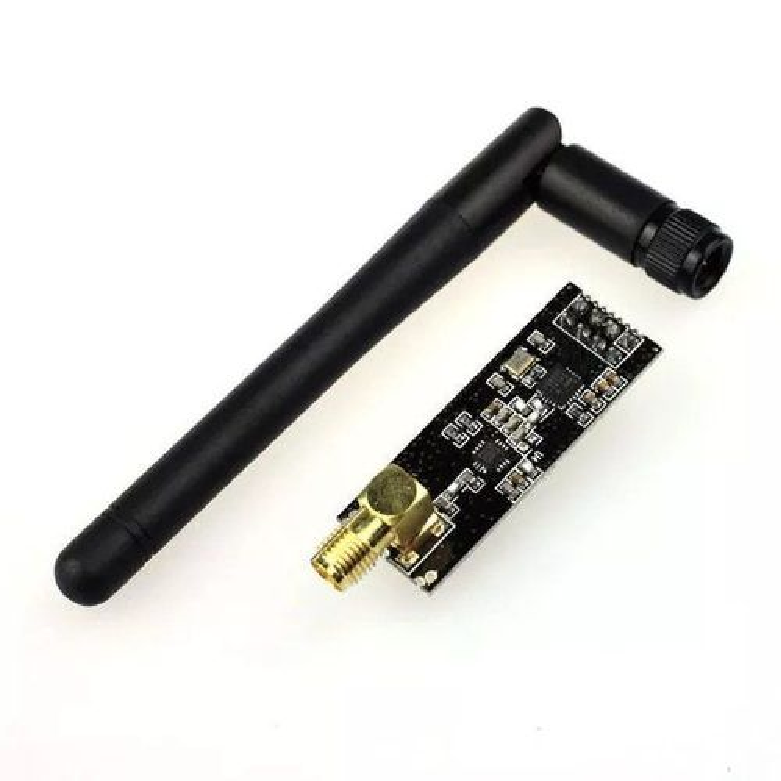
\includegraphics[scale = 0.6]{nrf24.pdf}
    \caption{Módulo \emph{Wi-fi} NRF24L01, utilizado para realizar a comunicação entre os totens.}
    \label{nrf24}
\end{figure}


    \subsection{Comparador de velocidade}
    O sistema de controle também é responsável por fazer uma comparação entre a velocidade do veículo que o mesmo recebe do rádio \emph{BladeRF}, com a velocidade máxima permitida da via, que normalmente é imposta pelo órgão de transito local.

    \subsection{Captura}
    Caso o veiculo monitorado esteja acima da velocidade permitida, é realizado uma estimativa de tempo para o veículo chegar na região de captura da câmera, mostrada na Figura \ref{camera}.
    
    Para realizar a escolha do modelo da câmera a ser utilizada foi primeiro determinado a faixa de distâncias que seriam possível realizar a captura da imagem, então estipulo-se a captura para uma distância de 7-10 m do radar. Tendo esse cálculo em vista foi levantado quais os fatores seriam determinantes para conseguir realizar a detecção e reconhecimento da placa do carro à distância determinada, e chegou-se a conclusão que os fatores que mais influenciariam na escolha seriam o tamanho de sua lente e também o diâmetro do sensor utilizado pela aparelho, pois esses dois fatores influenciam no ângulo de abertura da câmera, e como a distância de captura é considerável, quanto menor for o ângulo de abertura maior será a resolução da imagem captada. Outro fator importante é a utilização de uma lente varifocal, pois está possibilita um ajuste automático do foco da lente de acordo com que os objetos se aproximam ou afastam dela. 
    
    
    Para sabermos o tempo em que a câmera deve tirar a foto, será feito um cálculo de acordo com a posição, que é estimada fixando uma região na via para onde será enviado o sinal eletromagnético, e de acordo com a velocidade do veículo, que  será calculado no mesmo momento que a posição. Com esses dados se torna possível estimar o tempo que o veiculo demorará para passar na região em que a câmera está realizando a gravação da via, realizando a captura da imagem com o carro infrator devidamente posicionado.
    \begin{figure}[H]
    \centering
    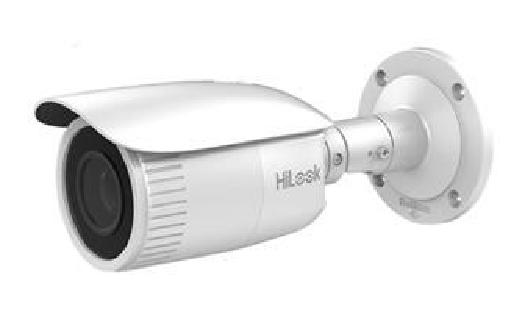
\includegraphics[scale = 0.8]{camera.pdf}
    \caption{Câmera IPC-B620H-V/Z responsável pela captura da traseira do veículo para reconhecimento da placa.}
    \label{camera}
\end{figure}
    \subsection{Envio de dados para o servidor}
    Para realizar o envio de dados para o servidor foi realizado previamente um estudo de caso para as rodovias brasileiras em geral, e notou-se que segundo o Departamento Nacional de Infraestrutura e Transporte (DNIT) o fluxo médio das grandes rodovias é de aproximadamente 60 mil veículos por dia, de onde cerca de somente 0.5\% desse veículos geram infrações, resultando em uma média de 300 veículos infratores por dia. Foi estipulado pelo grupo o envio de duas imagens com resolução de 2 \emph{megapixels}, estimando que o pacote de dados após as imagens serem transformadas em \emph{base64} ficaria em torno de 6 \emph{MBytes}. Com esses dados pode-se calcular que o volume médio de dados enviados para o servidor seria de 1800 \emph{MBytes} por dia, estimando que a conexão com servidor ocorra sem quedas durante o dia. A taxa de transmissão miníma para garantir a entrega de todos os dados é de 20.84 \emph{KBytes/s}. A princípio foi estipulado para o projeto o uso de um módulo \emph{General Packet Radio Services - GPRS} para transmissão desses dados, porém o mesmo tem uma capacidade máxima de transmissão de 10.63 \emph{KBytes/s}, e por este fato optou-se por conectar um \emph{switch}  como representado na Figura \ref{switch} a uma rede de acesso local para garantir o envio e recebimento dos dados. % Completar justificativa switch
        \begin{figure}[H]
            \centering
            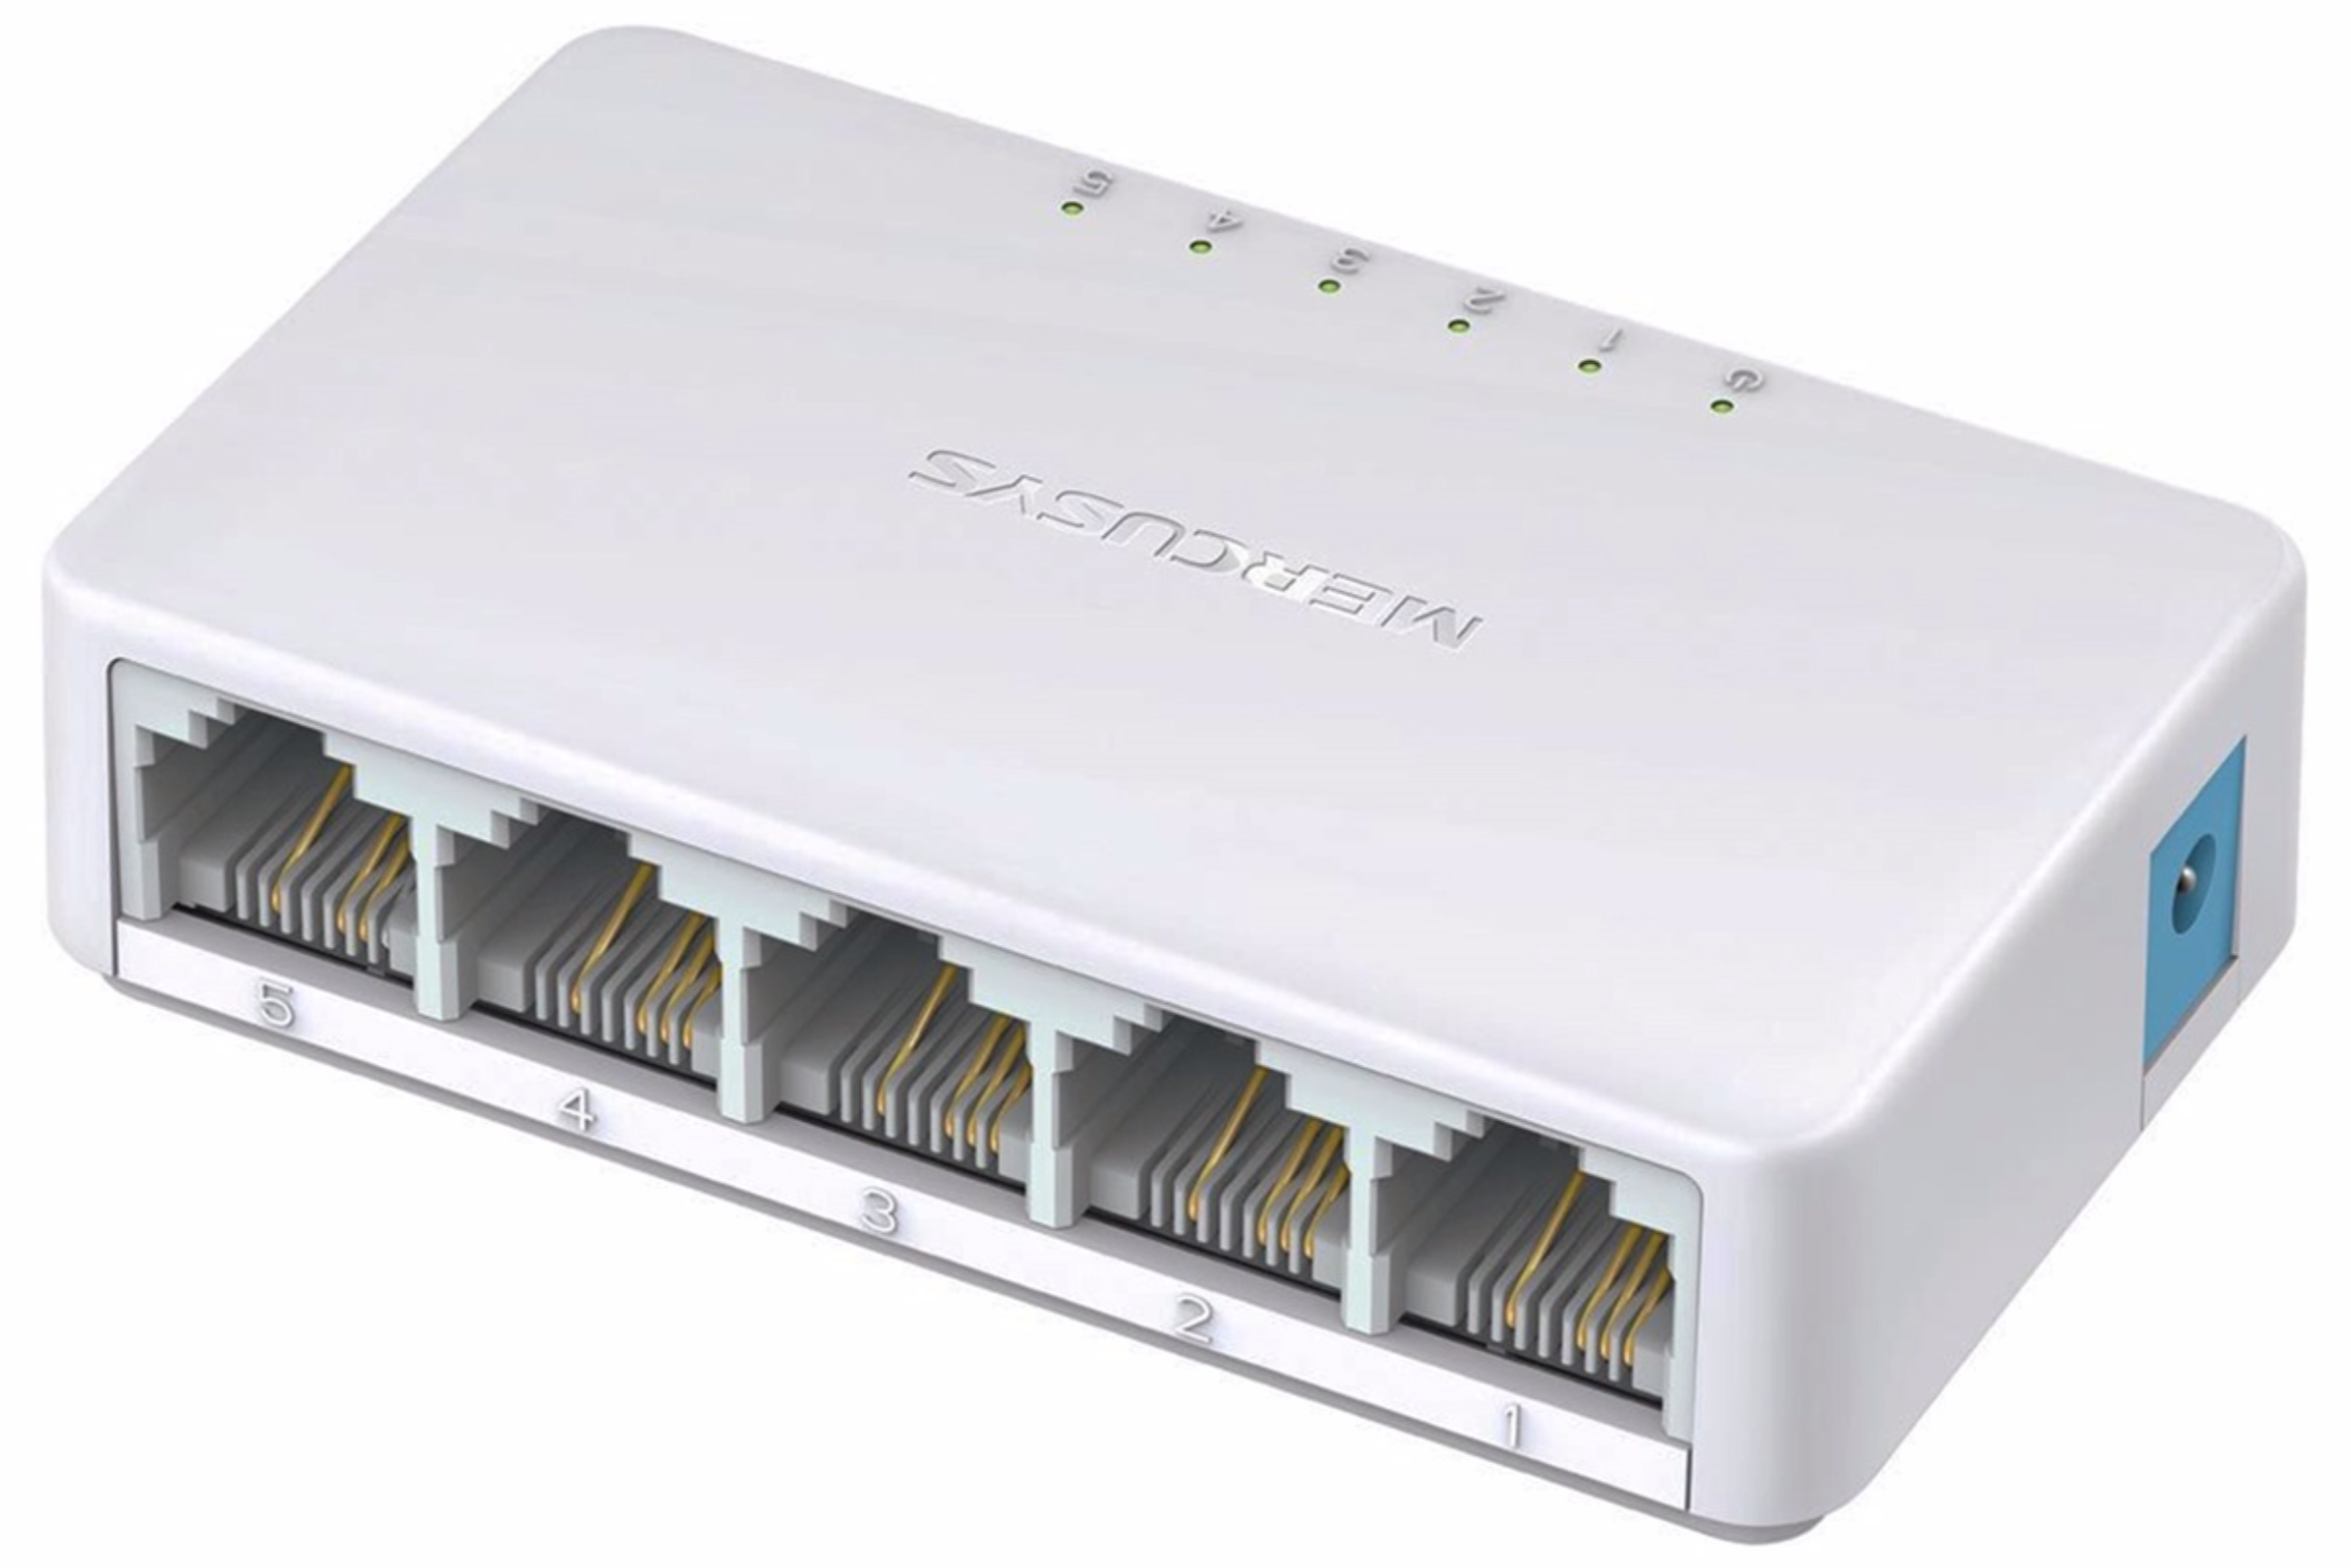
\includegraphics[scale=0.15]{switch.png}
            \caption{Módulo \emph{switch} utilizado para transmissão e recepção dos dados com o servidor e com a câmera.}
            \label{switch}
        \end{figure}

\section{Processamento de Imagens}

Este processo tem como objetivo "binarizar/simplificar" e extrair a placa do veículo da imagem capturada pela câmera para facilitar no reconhecimento de caracteres da placa que será feito pelo servidor. Para isso serão utilizadas algumas técnicas como mostrado no diagrama na Figura \ref{processamento}.


\begin{figure}[H]
    \centering
    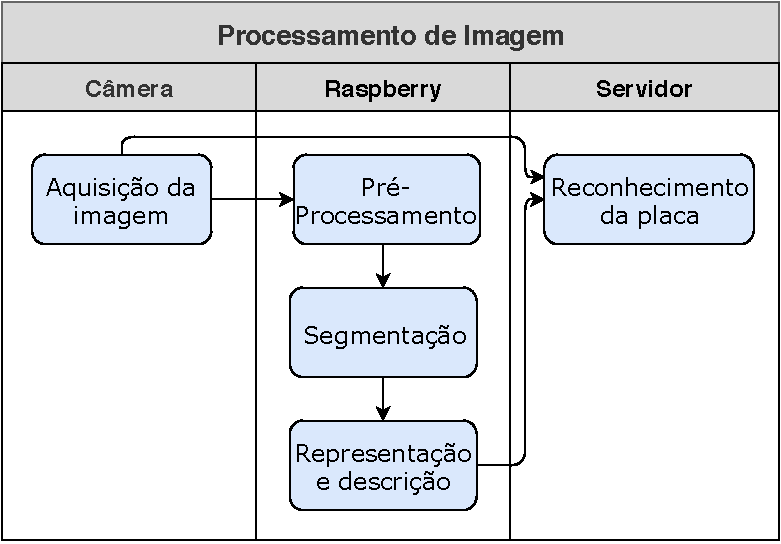
\includegraphics[scale=0.85]{processamento_imagem.pdf}
    \caption{Diagrama dos processos realizados pelo sistema de processamento de imagem.}
    \label{processamento}
\end{figure}

   A aquisição de imagem acontecerá pela câmera, que fará a captura do veículo e enviará para a \emph{Raspberry} dar início ao pré processamento.  
   
\begin{itemize}
    \item Pré - Processamento
    \item Segmentação
    \item Representação e descrição
\end{itemize}



\section{Sistema de comunicação}
Para realizar a sincronização dos sinais enviados e recebidos, o sistema de comunicação tem como objetivo estabelecer quais protocolos serão utilizados entre a comunicação dos módulos, de modo que os mesmos fossem adequados para o escopo de comunicação de cada um.

As escolhas para os mesmos foram baseadas na disponibilidade de protocolos  de comunicação de cada um dos módulos e também no desempenho dos protocolos, de acordo com a Figura \ref{diagrama_logico}.


\begin{figure}[H]
    \centering
    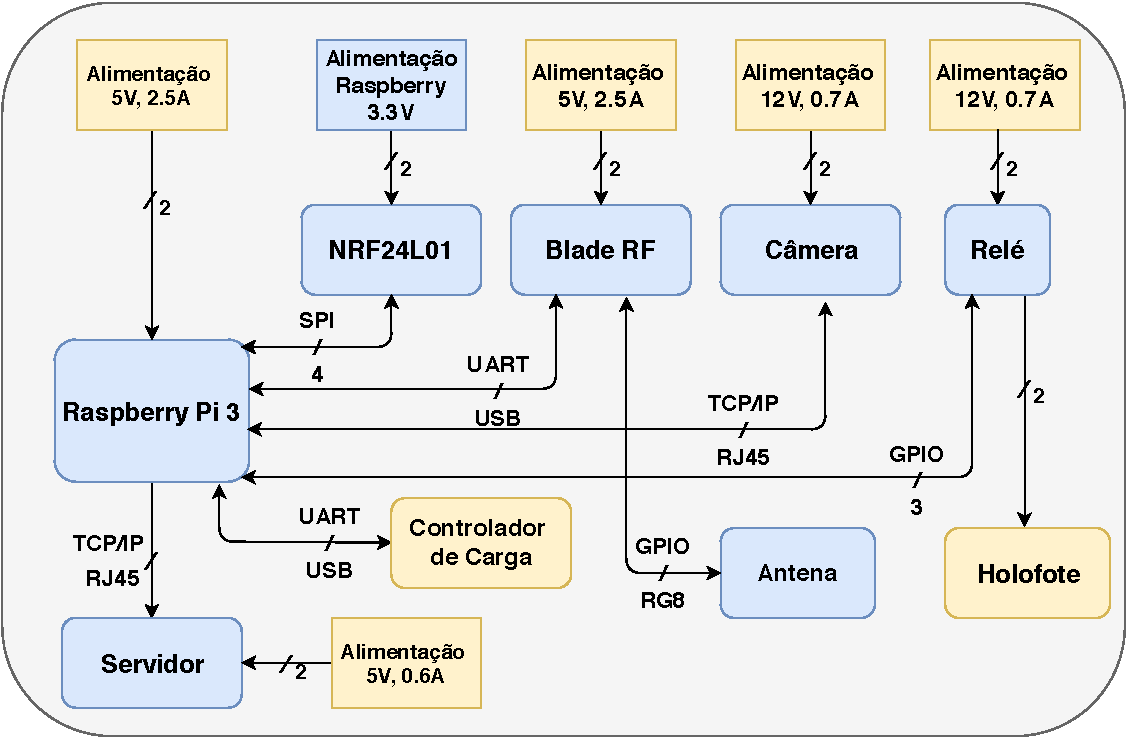
\includegraphics[scale=0.7]{Diagrama_Logico.pdf}
    \caption{Diagrama geral da comunicação e alimentação dos módulos presentes no sistema do radar. }
    \label{diagrama_logico}
\end{figure}



\subsection{\emph{Serial Peripheral Interface - SPI}}
    O SPI é um protocolo de comunicação serial síncrono que fará a conexão entre a \emph{Raspberry Pi} e o módulo \emph{Wifi NRF24L01}. Este protocolo possui dentre suas características a arquitetura mestre-escravo, sendo o mestre a \emph{Raspberry Pi} e escravo o módulo \emph{NRF24L01}, o modo de comunicação \emph{full-duplex}, sendo possível tanto o mestre transmitir informações para o escravo como o escravo também pode transmitir informação para o mestre, e possuir uma taxa máxima de 2 Mbps, sendo esta velocidade bastante alta em relação a outros protocolos de comunicação.
    Utilizar o módulo \emph{NRF24L01} foi determinado pelo fato dele ser pequeno, de baixo consumo de energia, pelas vantagens do seu protocolo de comunicação ser SPI e por conter uma antena externa que permite o sinal ser transmitido em até 1 Km de distância.
    As conexões entre a \emph{Raspeberry} e o módulo NRF é visto na Figura \ref{fritizingnrf} e na Tabela \ref{tabelanrf}.
    
    \begin{figure}[H]
    \centering
    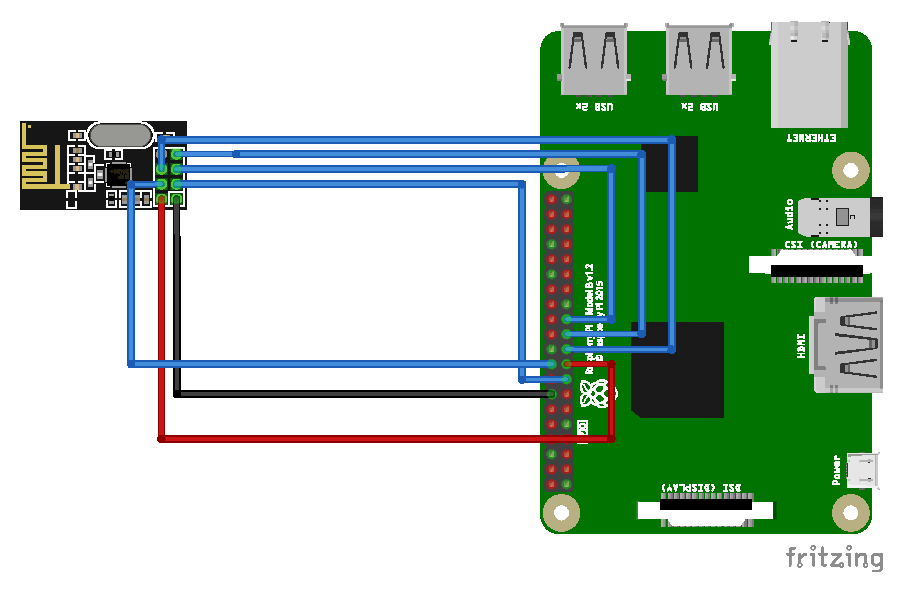
\includegraphics[scale=0.6]{fritzingnrf.pdf}
    \caption{Esquemático entre a \emph{Raspberry} e o módulo NRF24, mostrando as conexões de cada pino entre eles.}
    \label{fritizingnrf}
\end{figure}

    
  \begin{table}[h]
 \centering
% distancia entre a linha e o texto
 {\renewcommand\arraystretch{1.25}
 \caption{Conexão entre a \emph{Raspberry} e o módulo NRF24 por pinagem.}
 \begin{tabular}{ l l }
  \cline{1-1}\cline{2-2}  
    \multicolumn{1}{|p{3.850cm}|}{NRF24L01 \centering } &
    \multicolumn{1}{p{4.217cm}|}{\emph{Raspberry Pi 3} \centering }
  \\  
  \cline{1-1}\cline{2-2}  
    \multicolumn{1}{|p{3.850cm}|}{VCC \centering } &
    \multicolumn{1}{p{4.217cm}|}{17 (3.3V) \centering }
  \\  
  \cline{1-1}\cline{2-2}  
    \multicolumn{1}{|p{3.850cm}|}{GND \centering } &
    \multicolumn{1}{p{4.217cm}|}{25  \centering }
  \\  
  \cline{1-1}\cline{2-2}  
    \multicolumn{1}{|p{3.850cm}|}{CE \centering } &
    \multicolumn{1}{p{4.217cm}|}{15 \centering }
  \\  
  \cline{1-1}\cline{2-2}  
    \multicolumn{1}{|p{3.850cm}|}{CS \centering } &
    \multicolumn{1}{p{4.217cm}|}{18 \centering }
  \\  
  \cline{1-1}\cline{2-2}  
    \multicolumn{1}{|p{3.850cm}|}{SCK \centering } &
    \multicolumn{1}{p{4.217cm}|}{23 \centering }
  \\  
  \cline{1-1}\cline{2-2}  
    \multicolumn{1}{|p{3.850cm}|}{MOSI \centering } &
    \multicolumn{1}{p{4.217cm}|}{19 \centering }
  \\  
  \cline{1-1}\cline{2-2}  
    \multicolumn{1}{|p{3.850cm}|}{MISO \centering } &
    \multicolumn{1}{p{4.217cm}|}{21 \centering }
  \\  
  \cline{1-1}\cline{2-2}  
    \multicolumn{1}{|p{3.850cm}|}{IRQ \centering } &
    \multicolumn{1}{p{4.217cm}|}{- \centering }
  \\  
  \hline
\label{tabelanrf}
 \end{tabular} }
\end{table}  


\subsection{\emph{Universal Synchronous Receiver/Transmitter - UART}}
    Para realizar a comunicação entre o microcontrolador \emph{Raspberry Pi 3} e o rádio \emph{BladeRF}, e o controlador de carga foi utilizado o protocolo de comunicação UART, isso devido ao seu alto índice de mobilidade na transmissão dos dados de um módulo para o outro. Para conseguir isso o protocolo realiza a transmissão e recepção dos dados de forma serial e assíncrona, isso significa que não é necessário que os módulos aos quais irão se comunicar através do protocolo UART estejam sincronizados no mesmo ciclo de \emph{clock} e que tanto a recepção (RX) como a transmissão (TX) possuem somente um cabo para se comunicar com o outro módulo, além disso a mesma possibilita uma comunicação simultânea entre os dois módulos ou seja, uma transmissão \emph{full-duplex}. Através dessa mobilidade acaba-se tornando uma boa opção para realizar a transferência de dados entre os módulos citados.
    
    


\subsection{\emph{General Porpouse Input/Output - GPIO}}

Os GPIOs são portas de entradas e saídas digitas, podendo ser programadas e controladas para comunicações entre módulos e controle de estado de componentes. A \emph{Raspberry} possui no total 46 pinos GPIO, possuindo uma tensão em nível lógico alto de 3.3V, e em nível lógico baixo de 0V. A Figura \ref{datasheet} mostra a numeração dos pinos e suas respectivas comunicações.

\begin{figure}[H]
    \centering
    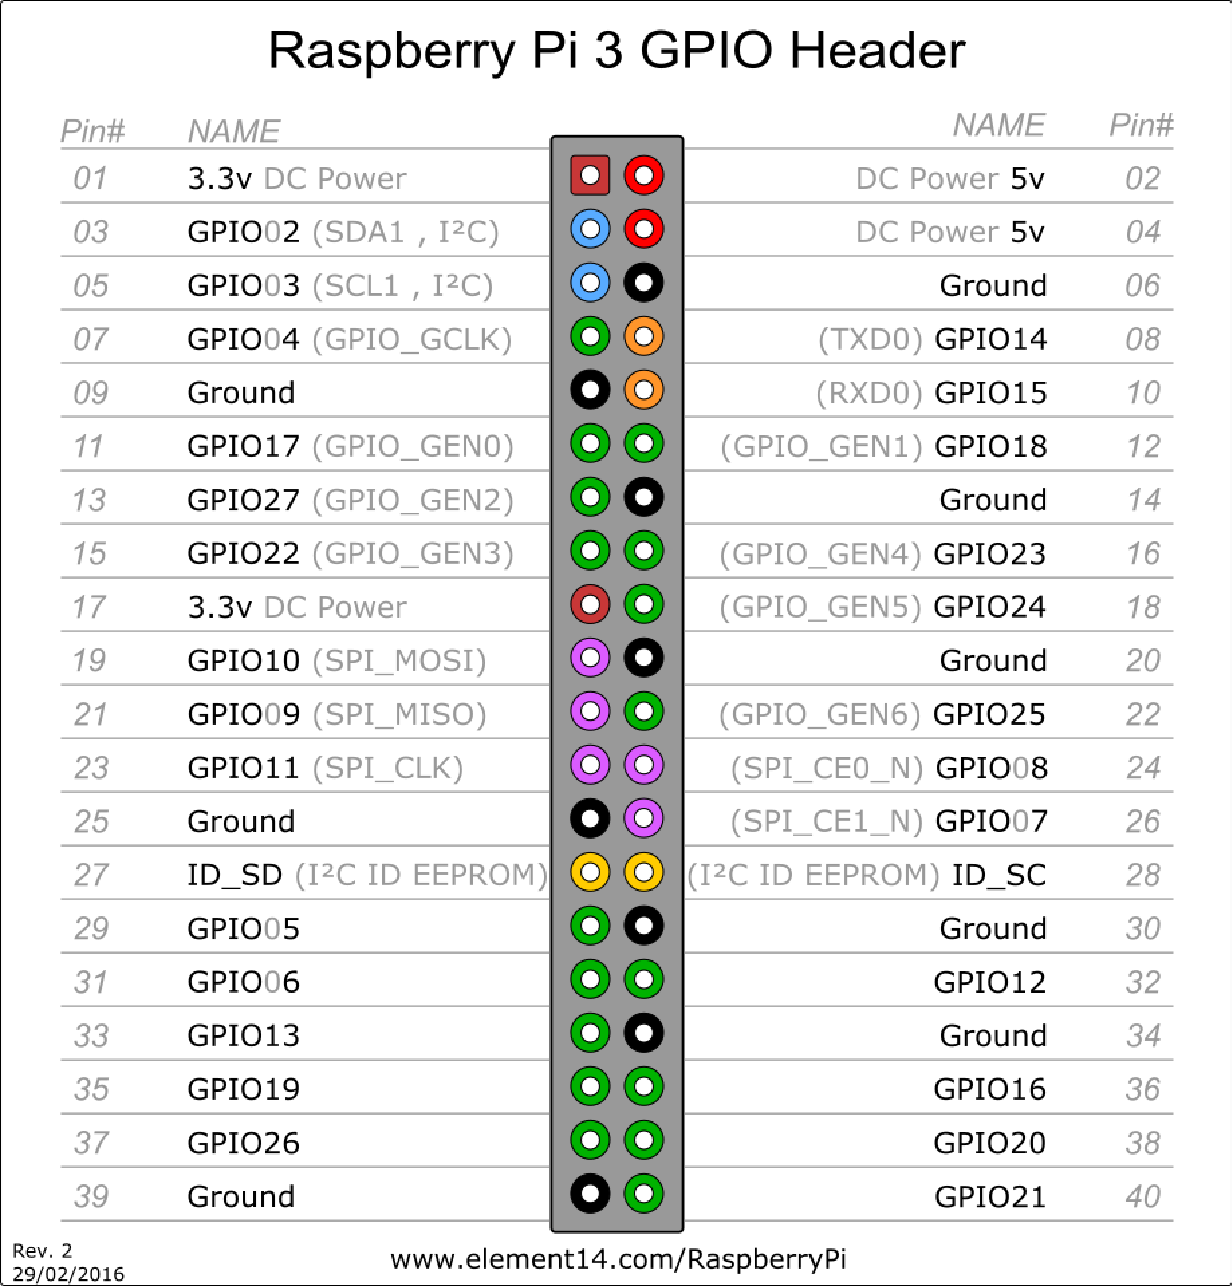
\includegraphics[scale=0.5]{datasheet.pdf}
    \caption {Pinagem da placa \emph{Raspberry PI 3} com todos os protocolos de comunicação e seus respectivos pinos.}
    \label{datasheet}
\end{figure}


A comunicação por GPIO irá realizar o controle do holofote através de um relé, onde o mesmo fará o chaveamento de quando o holofote vai iluminar ou não. Neste caso, será determinado um período de tempo em que quando o relé receber determinado sinal vindo da \emph{Raspberry} o mesmo irá para um nível lógico alto, fazendo com que seja acionado um sinal luminoso. Após o período o relé irá voltar para o nível lógico baixo e ficara a espera do estimulo para repetir este processo.  As conexões entre a \emph{Raspberry} e o módulo relé é visto na Figura \ref{fritizingrele} e na Tabela \ref{tabelarele}.

    \begin{figure}[H]
    \centering
    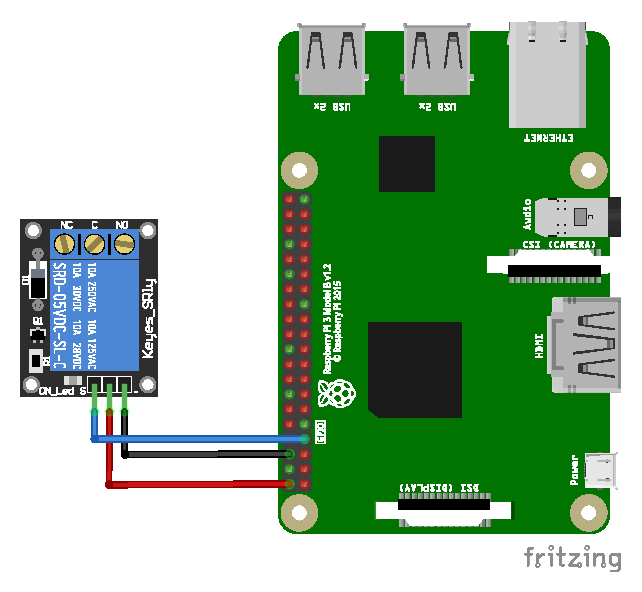
\includegraphics[scale=0.6]{fritzingrele.pdf}
    \caption{Esquemático entre a \emph{Raspberry} e o módulo relé, mostrando as conexões de cada pino entre eles.}
    \label{fritizingrele}
\end{figure}

  \begin{table}[h]
 \centering
% distancia entre a linha e o texto
 {\renewcommand\arraystretch{1.25}
 \caption{Conexão entre a \emph{Raspberry} e o relé por pinagem.}
 \begin{tabular}{ l l }
  \cline{1-1}\cline{2-2}  
    \multicolumn{1}{|p{3.850cm}|}{Rele \centering } &
    \multicolumn{1}{p{4.217cm}|}{\emph{Raspberry Pi 3} \centering }
  \\  
  \cline{1-1}\cline{2-2}  
    \multicolumn{1}{|p{3.850cm}|}{VCC \centering } &
    \multicolumn{1}{p{4.217cm}|}{02 (5V) \centering }
  \\  
  \cline{1-1}\cline{2-2}  
    \multicolumn{1}{|p{3.850cm}|}{GND \centering } &
    \multicolumn{1}{p{4.217cm}|}{06  \centering }
  \\  
  \cline{1-1}\cline{2-2}  
    \multicolumn{1}{|p{3.850cm}|}{IN1 \centering } &
    \multicolumn{1}{p{4.217cm}|}{07 \centering }
  \\  
   \hline
\label{tabelarele}
 \end{tabular} }
\end{table}  


\subsection{ \emph{Transmission Control Protocol/Internet Protocol - TCP/IP}}
Utilizado para se comunicar com a rede de computadores o protocolo TCP/IP é um protocolo que é dividido em camadas, sendo elas:
\begin{itemize}
    \item Camada de Aplicação: É a interface entre o usuário e o sistema operacional.
    \item Camada de Transporte (TCP): Roteia o caminho de uma máquina a outra.
    \item Camada de Internet (IP): Contém os dados e o endereçamento do IP.
    \item Camada de Acesso à Rede: Contem todas as informações físicas a respeito da transmissão dos dados.
    
\end{itemize}

A utilização desse tipo de arquitetura possibilita o que chamamos de encapsulamento de dados, que faz com que as informações de uma camada superior sejam adicionadas no final do pacote recebido pela mesma, criando assim uma espécie de cabeçalho que garante a transmissão e recepção de dados com a rede.
Este protocolo será responsável por fazer a comunicação da \emph{Raspberry} com a câmera e o servidor. Eles serão conectados ao \emph{switch} pelo fato da \emph{Raspberry} conter apenas uma porta \emph{ethernet}, e para conexão entre eles será utilizado cabo RJ45.

